\section{基本内容及主要方法}

\subsection{行人重识别基线模型}

\begin{frame}{行人重识别基线模型}
\begin{figure}
    \centering
    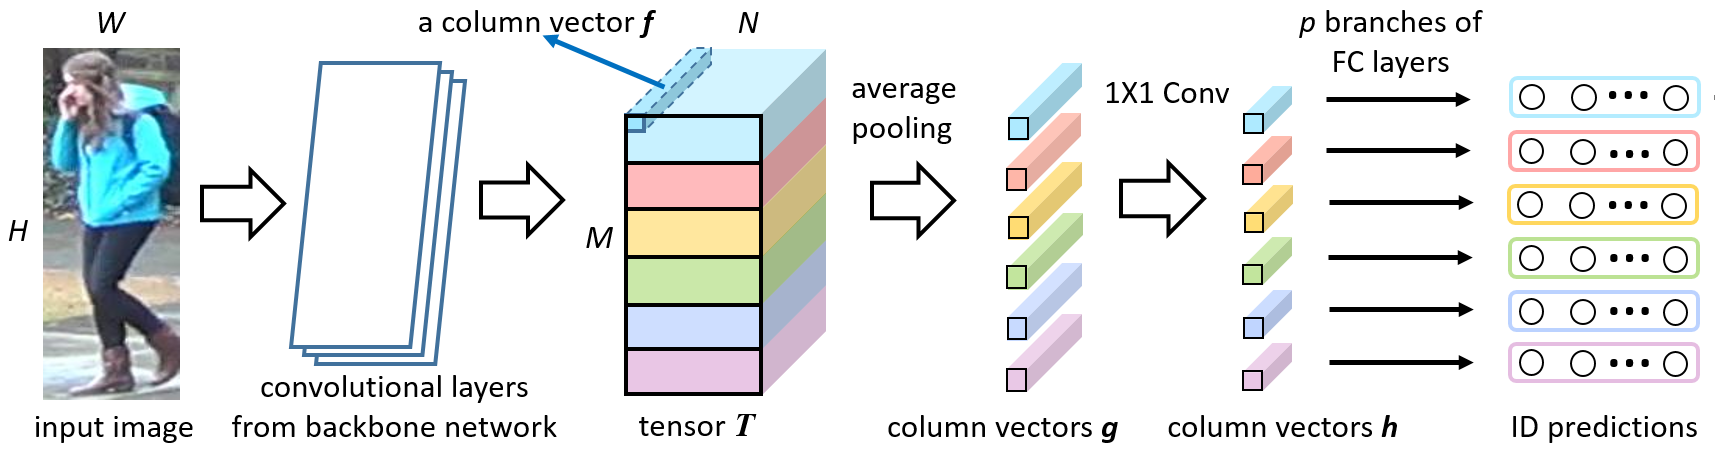
\includegraphics[width=10cm]{structure}
\end{figure}
\end{frame}

\subsection{强化学习模型}

\begin{frame}{用于多摄像头选择的强化学习模型}
\begin{block}

    强化学习模型使用了经典的 Q-Learning 算法,对智能体进行训练。
    \vskip 1em
    \begin{table}
        \begin{tabular}{rl}
            当前状态集合 & $S=\left\{\boldsymbol{s}\,\middle\vert\,\boldsymbol{s}\in\mathbb{R}^{N}, s_i\in\{0, 1\}\right\}$ \\[1em]
            智能体动作集合 & $A=\left\{\boldsymbol{a}\,\middle\vert\,\boldsymbol{a}\in\mathbb{R}^N,\boldsymbol{a}_i \in \{0,1\}\right\}$\\[1em]
            状态转移概率 & $\pi\left(\boldsymbol{s}^t\,\middle\vert\,\boldsymbol{s}^{t-1}, \boldsymbol{a}\right)\equiv1$\\[1em]
            环境的反馈 & $r=\mathcal{E}\left[\mathcal{F}\left(\mathcal{I}^{(t+1)}\right)\right]-\mathcal{E}\left[\mathcal{F}\left(\mathcal{I}^{(t)}\right)\right]$\\[1em]
            当前状态 $S$ 的长期价值 & $V:\,S\mapsto\mathbb{R}^N$\\[1em]
            智能体应对当前状态的策略 & $P:\,V\mapsto A$
        \end{tabular}
    \end{table}
\end{block}
\end{frame}

\subsection{多CPU集群}

\begin{frame}{面向 CPU 集群的分布式深度学习训练框架}
    \begin{figure}
        \centering
        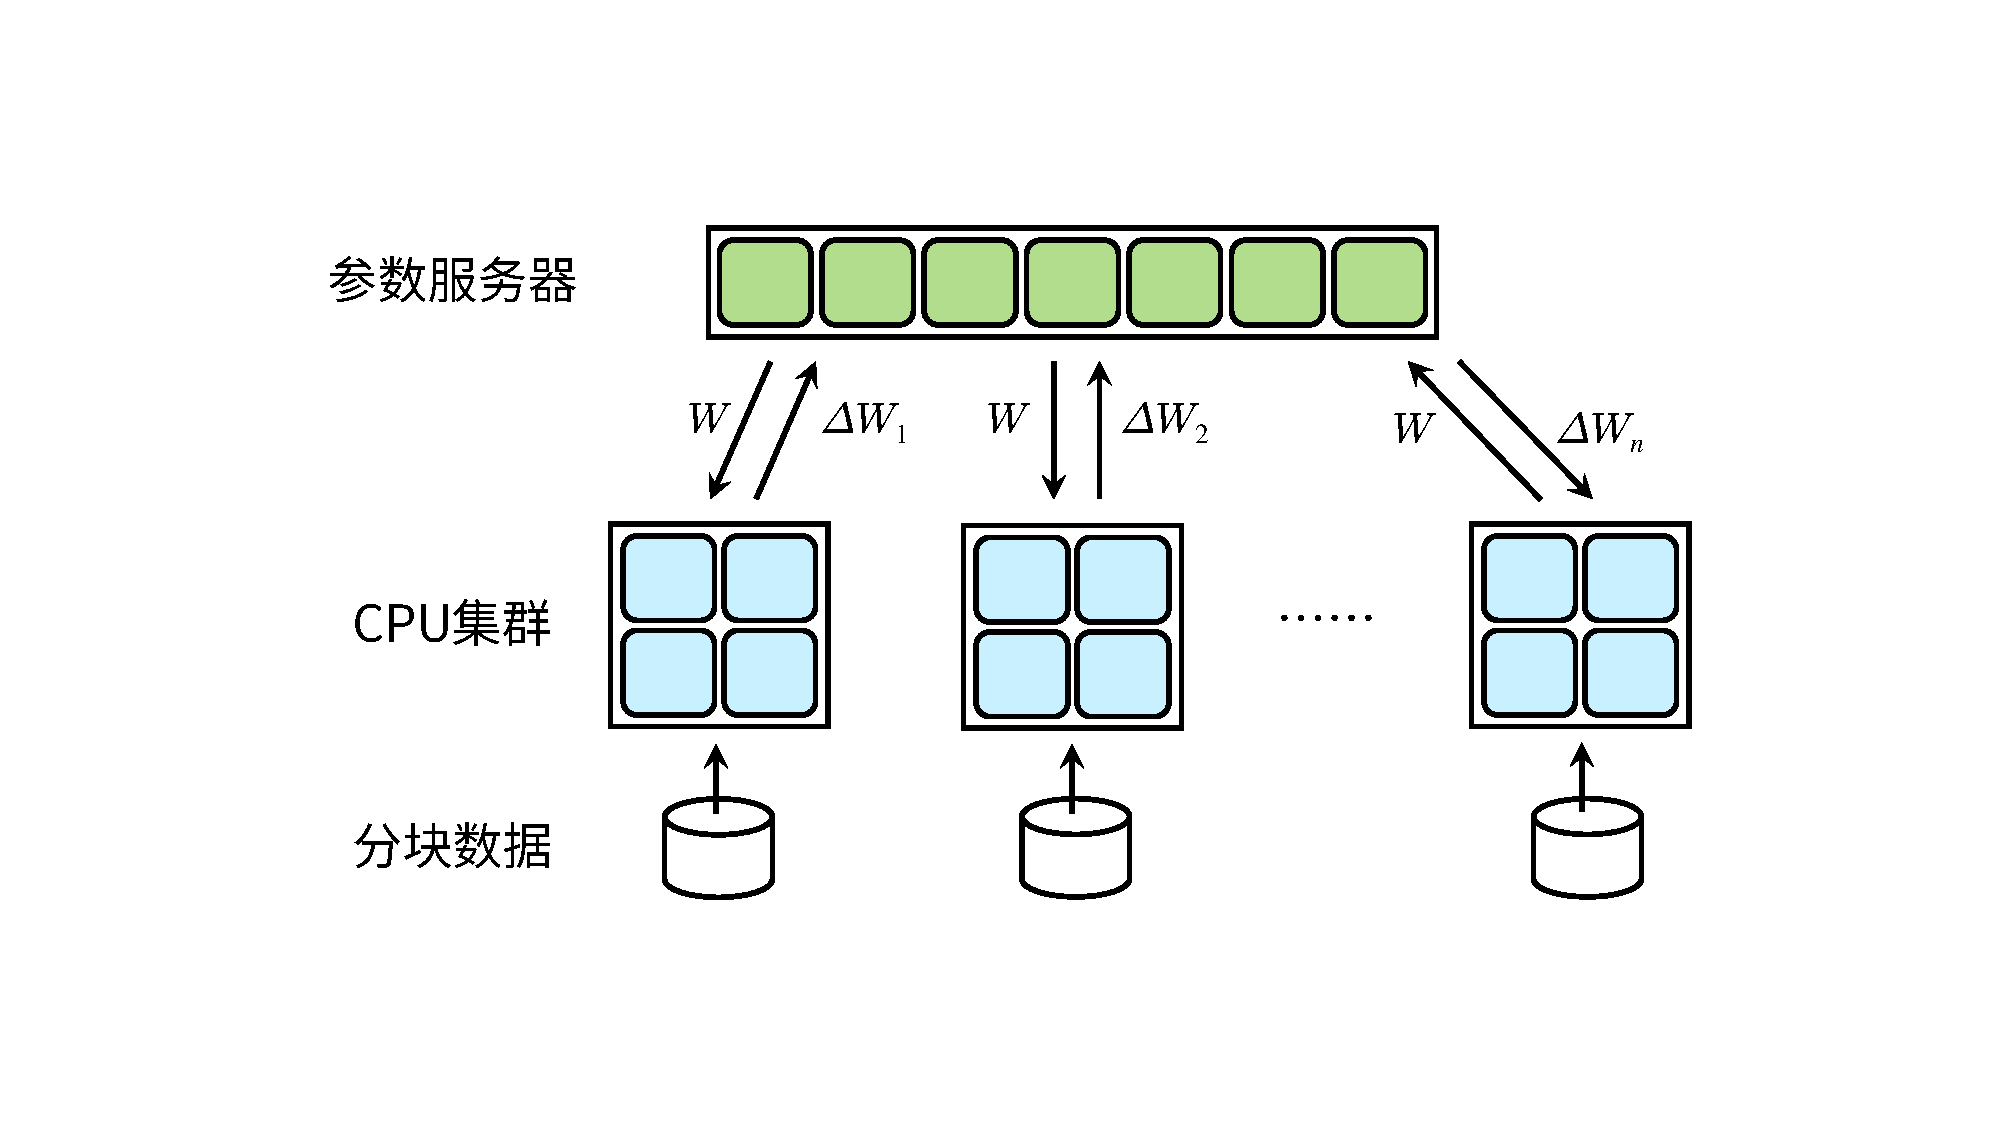
\includegraphics[width=0.7\textwidth]{dist}
    \end{figure}
\end{frame}